\documentclass[border=8pt]{standalone}
\usepackage{tikz}
\usetikzlibrary{arrows.meta,positioning,calc,fit}
\begin{document}
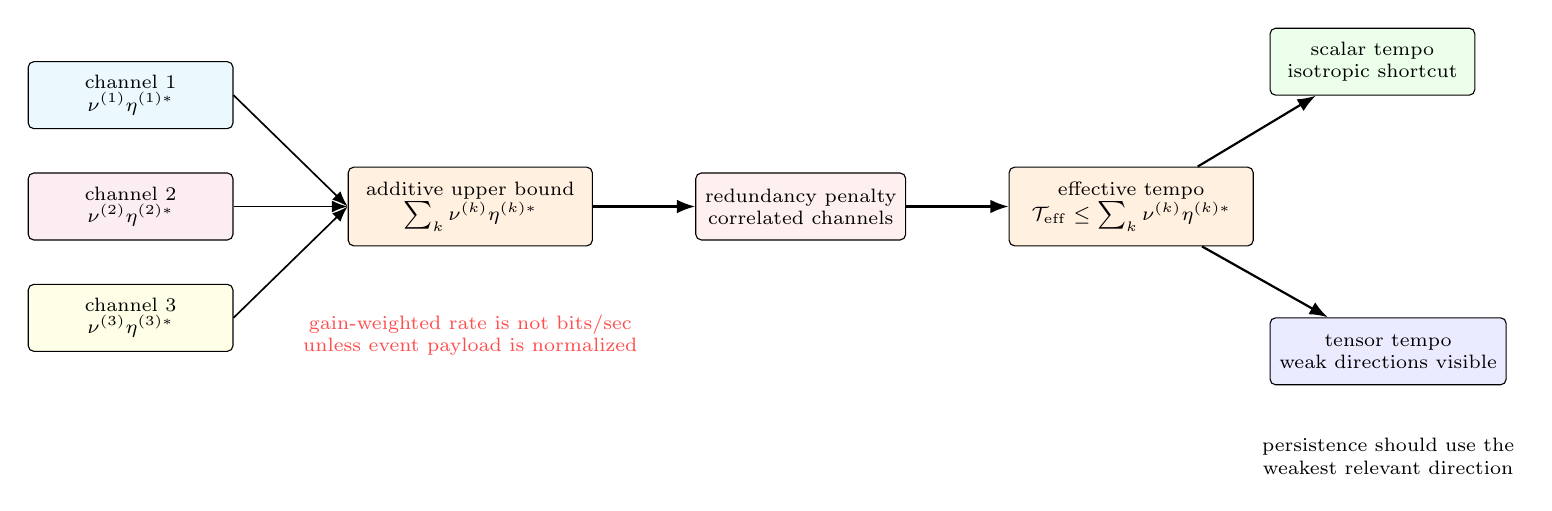
\begin{tikzpicture}[
  box/.style={draw, rounded corners=2pt, align=center, minimum width=2.6cm, minimum height=0.85cm, font=\scriptsize},
  funnel/.style={draw, rounded corners=2pt, align=center, minimum width=3.1cm, minimum height=1.0cm, font=\scriptsize, fill=orange!12},
  note/.style={align=center, font=\scriptsize},
  arr/.style={-Latex, thick},
  thinarr/.style={-Latex, semithick}
]

\node[box, fill=cyan!8] (c1) {channel 1\\$\nu^{(1)}\eta^{(1)*}$};
\node[box, fill=purple!7, below=0.55cm of c1] (c2) {channel 2\\$\nu^{(2)}\eta^{(2)*}$};
\node[box, fill=yellow!10, below=0.55cm of c2] (c3) {channel 3\\$\nu^{(3)}\eta^{(3)*}$};

\node[funnel, right=1.45cm of c2] (sum) {additive upper bound\\$\sum_k\nu^{(k)}\eta^{(k)*}$};
\draw[thinarr] (c1.east) -- (sum.west);
\draw[thinarr] (c2.east) -- (sum.west);
\draw[thinarr] (c3.east) -- (sum.west);

\node[box, fill=red!6, right=1.3cm of sum] (red) {redundancy penalty\\correlated channels};
\node[funnel, right=1.3cm of red] (eff) {effective tempo\\$\mathcal T_{\rm eff}\leq\sum_k\nu^{(k)}\eta^{(k)*}$};
\draw[arr] (sum) -- (red);
\draw[arr] (red) -- (eff);

\node[box, fill=green!8, above right=0.9cm and 0.2cm of eff] (scalar) {scalar tempo\\isotropic shortcut};
\node[box, fill=blue!8, below right=0.9cm and 0.2cm of eff] (tensor) {tensor tempo\\weak directions visible};
\draw[arr] (eff) -- (scalar);
\draw[arr] (eff) -- (tensor);

\node[note, below=0.75cm of sum, text=red!70] {gain-weighted rate is not bits/sec\\unless event payload is normalized};
\node[note, below=0.55cm of tensor] {persistence should use the\\weakest relevant direction};

\end{tikzpicture}
\end{document}
